\documentclass[10pt,fleqn]{article} % Default font size and left-justified equations
\usepackage[%
    pdftitle={CIN : Cinématique du solide},
    pdfauthor={Xavier Pessoles}]{hyperref}

%%%%%%%%%%%%%%%%%%%%%%%%%%%%%%%%%%%%%%%%%
% Original author:
% Mathias Legrand (legrand.mathias@gmail.com) with modifications by:
% Vel (vel@latextemplates.com)
% License:
% CC BY-NC-SA 3.0 (http://creativecommons.org\newtheorem{rappelT}{Rappel}[section]/licenses/by-nc-sa/3.0/)
%%%%%%%%%%%%%%%%%%%%%%%%%%%%%%%%%%%%%%%%%

%----------------------------------------------------------------------------------------
%	VARIOUS REQUIRED PACKAGES AND CONFIGURATIONS
%----------------------------------------------------------------------------------------

\usepackage[top=2.5cm,bottom=2cm,left=2cm,right=2cm,headsep=40pt,a4paper]{geometry} % Page margins

\usepackage{graphicx} % Required for including pictures
\graphicspath{{images/}} % Specifies the directory where pictures are stored
\usepackage{float}

\usepackage{lipsum} % Inserts dummy text

\usepackage{tikz} % Required for drawing custom shapes

\usepackage[french]{babel} % English language/hyphenation
\frenchbsetup{StandardLists=true} % Pour éviter la collision babel enumitem pour les listes

\usepackage{enumitem} % Customize lists
\setlist{nolistsep} % Reduce spacing between bullet points and numbered lists

\usepackage{booktabs} % Required for nicer horizontal rules in tables

\usepackage{colortbl} % Couleur dans les tableaux

\usepackage{xcolor} % Required for specifying colors by name
%\definecolor{ocre}{RGB}{243,102,25} % Define the orange color used for highlighting throughout the book
\definecolor{ocre}{RGB}{49,133,156} % Couleur ''bleue''
\definecolor{violetf}{RGB}{112,48,160} % Couleur ''violet''
\usepackage{enumitem}
\usepackage{pifont} % Pour les dinglist
\usepackage{multicol}
\usepackage{array} % Centrage vertical dans les tableaux

%----------------------------------------------------------------------------------------
%	FONTS
%----------------------------------------------------------------------------------------

\usepackage{avant} % Use the Avantgarde font for headings
%\usepackage{times} % Use the Times font for headings
%\usepackage{mathptmx} % Use the Adobe Times Roman as the default text font together with math symbols from the Sym­bol, Chancery and Com­puter Modern fonts
\usepackage[adobe-utopia]{mathdesign}
\usepackage{microtype} % Slightly tweak font spacing for aesthetics
\usepackage[utf8]{inputenc} % Required for including letters with accents
\usepackage[T1]{fontenc} % Use 8-bit encoding that has 256 glyphs

%----------------------------------------------------------------------------------------
%	BIBLIOGRAPHY AND INDEX
%----------------------------------------------------------------------------------------

\usepackage[style=alphabetic,citestyle=numeric,sorting=nyt,sortcites=true,autopunct=true,babel=hyphen,hyperref=true,abbreviate=false,backref=true,backend=biber]{biblatex}
\addbibresource{bibliography.bib} % BibTeX bibliography file
\defbibheading{bibempty}{}

\usepackage{calc} % For simpler calculation - used for spacing the index letter headings correctly
\usepackage{makeidx} % Required to make an index
\makeindex % Tells LaTeX to create the files required for indexing

%----------------------------------------------------------------------------------------
%	MAIN TABLE OF CONTENTS
%----------------------------------------------------------------------------------------

\usepackage{titletoc} % Required for manipulating the table of contents

\setcounter{tocdepth}{2}     % Dans la table des matieres
\setcounter{secnumdepth}{2}

\contentsmargin{0cm} % Removes the default margin

% Part text styling
\titlecontents{part}[0cm]
{\addvspace{20pt}\centering\large\bfseries}
{}
{}
{}

% Chapter text styling
\titlecontents{chapter}[1.25cm] % Indentation
{\addvspace{12pt}\large\sffamily\bfseries} % Spacing and font options for chapters
{\color{ocre!60}\contentslabel[\Large\thecontentslabel]{1.25cm}\color{ocre}} % Chapter number
{\color{ocre}}  
{\color{ocre!60}\normalsize\;\titlerule*[.5pc]{.}\;\thecontentspage} % Page number

% Section text styling
\titlecontents{section}[1.25cm] % Indentation
{\addvspace{3pt}\sffamily\bfseries} % Spacing and font options for sections
{\color{ocre!60}\contentslabel[\thecontentslabel]{1.25cm} \color{ocre}} % Section number
{\color{ocre}}
{\hfill\color{ocre!60}\thecontentspage} % Page number
[]

% Subsection text styling
\titlecontents{subsection}[1.25cm] % Indentation
{\addvspace{1pt}\sffamily\small} % Spacing and font options for subsections
{\contentslabel[\thecontentslabel]{1.25cm}} % Subsection number
{}
{\ \titlerule*[.5pc]{.}\;\thecontentspage} % Page number
[]


% Subsection text styling
\titlecontents{subsubsection}[1.25cm] % Indentation
{\addvspace{1pt}\sffamily\small} % Spacing and font options for subsections
{\contentslabel[\thecontentslabel]{1.25cm}} % Subsection number
{}
{\ \titlerule*[.5pc]{.}\;\thecontentspage} % Page number
[]

% List of figures
\titlecontents{figure}[0em]
{\addvspace{-5pt}\sffamily}
{\thecontentslabel\hspace*{1em}}
{}
{\ \titlerule*[.5pc]{.}\;\thecontentspage}
[]

% List of tables
\titlecontents{table}[0em]
{\addvspace{-5pt}\sffamily}
{\thecontentslabel\hspace*{1em}}
{}
{\ \titlerule*[.5pc]{.}\;\thecontentspage}
[]

%----------------------------------------------------------------------------------------
%	MINI TABLE OF CONTENTS IN PART HEADS
%----------------------------------------------------------------------------------------

% Chapter text styling
\titlecontents{lchapter}[0em] % Indenting
{\addvspace{15pt}\large\sffamily\bfseries} % Spacing and font options for chapters
{\color{ocre}\contentslabel[\Large\thecontentslabel]{1.25cm}\color{ocre}} % Chapter number
{}  
{\color{ocre}\normalsize\sffamily\bfseries\;\titlerule*[.5pc]{.}\;\thecontentspage} % Page number

% Section text styling
\titlecontents{lsection}[0em] % Indenting
{\sffamily\small} % Spacing and font options for sections
{\contentslabel[\thecontentslabel]{1.25cm}} % Section number
{}
{}

% Subsection text styling
\titlecontents{lsubsection}[.5em] % Indentation
{\normalfont\footnotesize\sffamily} % Font settings
{}
{}
{}

%----------------------------------------------------------------------------------------
%	PAGE HEADERS
%----------------------------------------------------------------------------------------

\usepackage{fancyhdr} % Required for header and footer configuration



\pagestyle{fancy}
 \renewcommand{\headrulewidth}{0pt}
 \fancyhead{}
 \fancyhead[L]{%
 \noindent\begin{minipage}[c]{2.6cm}%
 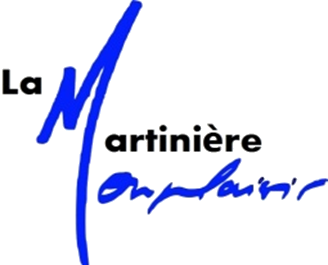
\includegraphics[width=2cm]{png/logo_lycee.png}%
 \end{minipage}}

\fancyhead[C]{\rule{8cm}{.5pt}}

 \fancyhead[R]{%
 \noindent\begin{minipage}[c]{3cm}
 \begin{flushright}
 \footnotesize{\textit{\textsf{\xxtete}}}%
 \end{flushright}
 \end{minipage}
}


\fancyfoot[C]{\rule{12cm}{.5pt}}
\renewcommand{\footrulewidth}{0.2pt}
\fancyfoot[C]{\footnotesize{\bfseries \thepage}}
\fancyfoot[L]{ 
\begin{minipage}[c]{.2\linewidth}
\noindent\footnotesize{{\xxauteur}}
\end{minipage}}


\fancyfoot[R]{\footnotesize{\xxpied}
\ifthenelse{\isodd{\value{page}}}{
\begin{tikzpicture}[overlay]
\node[shape=rectangle, 
      rounded corners = .25 cm,
	  draw= ocre,
	  line width=2pt, 
	  fill = ocre!10,
	  minimum width  = 2.5cm,
	  minimum height = 3cm,] at (\xxposongletx,\xxposonglety) {};
\node at (\xxposonglettext,\xxposonglety) {\rotatebox{90}{\textbf{\large\color{ocre}{\xxonglet}}}};
%{};
\end{tikzpicture}}{}
}
%
%
%
% Removes the header from odd empty pages at the end of chapters
\makeatletter
\renewcommand{\cleardoublepage}{
\clearpage\ifodd\c@page\else
\hbox{}
\vspace*{\fill}
\thispagestyle{empty}
\newpage
\fi}

\fancypagestyle{plain}{%
\fancyhf{} % vide l’en-tête et le pied~de~page.
%\fancyfoot[C]{\bfseries \thepage} % numéro de la page en cours en gras
% et centré en pied~de~page.
\fancyfoot[R]{\footnotesize{\xxpied}}
\fancyfoot[C]{\rule{12cm}{.5pt}}
\renewcommand{\footrulewidth}{0.2pt}
\fancyfoot[C]{\footnotesize{\bfseries \thepage}}
\fancyfoot[L]{ 
\begin{minipage}[c]{.2\linewidth}
\noindent\footnotesize{{\xxauteur}}
\end{minipage}}}



%----------------------------------------------------------------------------------------
%	THEOREM STYLES
%----------------------------------------------------------------------------------------

% Conflit avec la police adobe
%\usepackage{amsmath,amsfonts,amssymb,amsthm} % For math equations, theorems, symbols, etc
\usepackage{amsmath,amsthm}

\newcommand{\intoo}[2]{\mathopen{]}#1\,;#2\mathclose{[}}
\newcommand{\ud}{\mathop{\mathrm{{}d}}\mathopen{}}
\newcommand{\intff}[2]{\mathopen{[}#1\,;#2\mathclose{]}}
%\newtheorem{notation}{Notation}[chapter]
\newtheorem{notation}{Notation}[section]

% Boxed/framed environments
\newtheoremstyle{ocrenumbox}% % Theorem style name
{0pt}% Space above
{0pt}% Space below
{\normalfont}% % Body font
{}% Indent amount
{\small\bf\sffamily\color{ocre}}% % Theorem head font
{\;}% Punctuation after theorem head
{0.25em}% Space after theorem head
{\small\sffamily\color{ocre}\thmname{#1}\nobreakspace\thmnumber%{\@ifnotempty{#1}{}\@upn{#2}}% Theorem text (e.g. Theorem 2.1)
\thmnote{\nobreakspace\the\thm@notefont\sffamily\bfseries\color{black}---\nobreakspace#3.}} % Optional theorem note
\renewcommand{\qedsymbol}{$\blacksquare$}% Optional qed square


% Boite pour les corriges
\newtheoremstyle{correctionbox}% % Theorem style name
{0pt}% Space above
{0pt}% Space below
{\normalfont}% % Body font
{}% Indent amount
{\small\bf\sffamily\color{violet}}% % Theorem head font
{\;}% Punctuation after theorem head
{0.25em}% Space after theorem head
{\small\sffamily\color{ocre}\thmname{#1}\nobreakspace\thmnumber%{\@ifnotempty{#1}{}\@upn{#2}}% Theorem text (e.g. Theorem 2.1)
\thmnote{\nobreakspace\the\thm@notefont\sffamily\bfseries\color{black}---\nobreakspace#3.}} % Optional theorem note
\renewcommand{\qedsymbol}{$\blacksquare$}% Optional qed square



\newtheoremstyle{blacknumex}% Theorem style name
{5pt}% Space above
{5pt}% Space below
{\normalfont}% Body font
{} % Indent amount
{\small\bf\sffamily}% Theorem head font
{\;}% Punctuation after theorem head
{0.25em}% Space after theorem head
{\small\sffamily{\tiny\ensuremath{\blacksquare}}\nobreakspace\thmname{#1}\nobreakspace\thmnumber%{\@ifnotempty{#1}{}\@upn{#2}}% Theorem text (e.g. Theorem 2.1)
\thmnote{\nobreakspace\the\thm@notefont\sffamily\bfseries---\nobreakspace#3.}}% Optional theorem note

\newtheoremstyle{blacknumbox} % Theorem style name
{0pt}% Space above
{0pt}% Space below
{\normalfont}% Body font
{}% Indent amount
{\small\bf\sffamily}% Theorem head font
{\;}% Punctuation after theorem head
{0.25em}% Space after theorem head
{\small\sffamily\thmname{#1}\nobreakspace 
\thmnote{\nobreakspace\the\thm@notefont\sffamily\bfseries---\nobreakspace#3.}}% Optional theorem note

% Non-boxed/non-framed environments
\newtheoremstyle{ocrenum}% % Theorem style name
{5pt}% Space above
{5pt}% Space below
{\normalfont}% % Body font
{}% Indent amount
{\small\bf\sffamily\color{ocre}}% % Theorem head font
{\;}% Punctuation after theorem head
{0.25em}% Space after theorem head
{\small\sffamily\color{ocre}\thmname{#1}\nobreakspace%\thmnumber{\@ifnotempty{#1}{}\@upn{#2}}% Theorem text (e.g. Theorem 2.1)
\thmnote{\nobreakspace\the\thm@notefont\sffamily\bfseries\color{black}---\nobreakspace#3.}} % Optional theorem note
\renewcommand{\qedsymbol}{$\blacksquare$}% Optional qed square
\makeatother

% Environnement pour les titres de parties
\newtheoremstyle{partiebox} 
{0pt}% Space above
{0pt}% Space below
{\normalfont}% Body font
{}% Indent amount
{\small\bf\sffamily}% Theorem head font
{\;}% Punctuation after theorem head
{0.25em}% Space after theorem head




% Defines the theorem text style for each type of theorem to one of the three styles above
\newcounter{dummy} 
\numberwithin{dummy}{section}
\theoremstyle{ocrenumbox}
%\newtheorem{theoremeT}[dummy]{Théorème}
\newtheorem{theoremeT}[dummy]{Théorème}
\newtheorem{resultatT}[dummy]{Résultat}
\newtheorem{savoirT}[dummy]{Savoir}
\newtheorem{methodeT}[dummy]{Méthode}
\newtheorem{objectifT}[dummy]{Objectif}
%\newtheorem{problem}{Problem}[chapter]
\newtheorem{problem}{Problem}[section]
%\newtheorem{exerciseT}{Exercise}[chapter]
\newtheorem{exerciseT}{Exercice}[section]

\theoremstyle{blacknumex}
%\newtheorem{exampleT}{Example}[chapter]
\newtheorem{exempleT}{Exemple}[section]
\newtheorem{termT}{Terminal\\}[section]
\newtheorem{pyT}{Python\\}[section]
\newtheorem{sciT}{Scilab\\}[section]
\newtheorem{pseudoT}{Pseudo Code\\}[section]
\newtheorem{sqlT}{SQL\\}[section]

\theoremstyle{blacknumbox}
%\newtheorem{vocabulary}{Vocabulary}[chapter]
\newtheorem{vocabulary}{Vocabulaire}[section]
%\newtheorem{definitionT}{Definition}[section]
\newtheorem{definitionT}{Définition}[section]
\newtheorem{rappelT}{Rappel}[section]
\newtheorem{demoT}{Démonstration}[section]
\newtheorem{corollaryT}[dummy]{Corollaire}
\newtheorem{hypoT}{Hypothèse(s)}

\theoremstyle{ocrenum}
\newtheorem{proposition}[dummy]{Proposition}

\theoremstyle{partiebox}
\newtheorem{titrepartieT}[]{}
\newtheorem{titrechapitreT}[]{}

\theoremstyle{correctionbox}
\newtheorem{correctionT}[dummy]{\color{violet}{Correction}}

%----------------------------------------------------------------------------------------
%	DEFINITION OF COLORED BOXES
%----------------------------------------------------------------------------------------

\RequirePackage[framemethod=tikz]{mdframed} % Required for creating the theorem, definition, exercise and corollary boxes

% Theorem box
\newmdenv[skipabove=7pt,
skipbelow=7pt,
backgroundcolor=ocre!10,
linecolor=ocre,
innerleftmargin=5pt,
innerrightmargin=5pt,
innertopmargin=5pt,
leftmargin=0cm,
rightmargin=0cm,
innerbottommargin=5pt]{tBox}


% Correction
\newmdenv[skipabove=7pt,
skipbelow=7pt,
backgroundcolor=violet!10,
linecolor=violet,
innerleftmargin=5pt,
innerrightmargin=5pt,
innertopmargin=5pt,
leftmargin=0cm,
rightmargin=0cm,
innerbottommargin=5pt]{coBox}


% Exercise box	  
\newmdenv[skipabove=7pt,
skipbelow=7pt,
rightline=false,
leftline=true,
topline=false,
bottomline=false,
backgroundcolor=ocre!10,
linecolor=ocre,
innerleftmargin=5pt,
innerrightmargin=5pt,
innertopmargin=5pt,
innerbottommargin=5pt,
leftmargin=0cm,
rightmargin=0cm,
linewidth=4pt]{eBox}	

% Definition box
\newmdenv[skipabove=7pt,
skipbelow=7pt,
rightline=false,
leftline=true,
topline=false,
bottomline=false,
backgroundcolor=ocre!10,
linecolor=ocre,
innerleftmargin=5pt,
innerrightmargin=5pt,
innertopmargin=1pt,
leftmargin=0cm,
rightmargin=0cm,
linewidth=4pt,
innerbottommargin=0pt]{dBox}	

% Demonstration box
\newmdenv[skipabove=7pt,
skipbelow=7pt,
rightline=false,
leftline=true,
topline=false,
bottomline=false,
%backgroundcolor=ocre!10,
linecolor=ocre,
innerleftmargin=5pt,
innerrightmargin=5pt,
innertopmargin=0pt,
leftmargin=0cm,
rightmargin=0cm,
linewidth=4pt,
innerbottommargin=0pt]{demoBox}	

% Corollary box
\newmdenv[skipabove=7pt,
skipbelow=7pt,
rightline=false,
leftline=true,
topline=false,
bottomline=false,
linecolor=gray,
backgroundcolor=black!5,
innerleftmargin=5pt,
innerrightmargin=5pt,
innertopmargin=5pt,
leftmargin=0cm,
rightmargin=0cm,
linewidth=4pt,
innerbottommargin=5pt]{cBox}


% Hypothèses
\newmdenv[skipabove=7pt,
skipbelow=7pt,
rightline=false,
leftline=true,
topline=false,
bottomline=false,
linecolor=gray,
backgroundcolor=black!5,
innerleftmargin=5pt,
innerrightmargin=5pt,
innertopmargin=5pt,
leftmargin=0cm,
rightmargin=0cm,
linewidth=4pt,
innerbottommargin=5pt]{hyBox}


% Boite pour le titre de la partie (pBox)
\newmdenv[skipabove=7pt,
skipbelow=7pt,
rightline=true,
leftline=false,
topline=false,
bottomline=false,
linecolor=ocre,
backgroundcolor=none,
innerleftmargin=5pt,
innerrightmargin=5pt,
innertopmargin=5pt,
leftmargin=0cm,
rightmargin=0cm,
linewidth=4pt,
innerbottommargin=5pt]{pBox}

% Boite pour le titre du chapitre (chBox)
\newmdenv[skipabove=7pt,
skipbelow=7pt,
rightline=false,
leftline=true,
topline=false,
bottomline=false,
linecolor=ocre,
%backgroundcolor=black!5,
innerleftmargin=5pt,
innerrightmargin=5pt,
innertopmargin=5pt,
leftmargin=0cm,
rightmargin=0cm,
linewidth=4pt,
innerbottommargin=5pt]{chBox}


% Boite pour les exemples
\newmdenv[skipabove=7pt,
skipbelow=7pt,
rightline=false,
leftline=true,
topline=false,
bottomline=false,
linecolor=gray,
backgroundcolor=white,
innerleftmargin=5pt,
innerrightmargin=5pt,
innertopmargin=5pt,
leftmargin=0cm,
rightmargin=0cm,
linewidth=4pt,
innerbottommargin=5pt]{exBox}

% Boite pour le terminal
\newmdenv[skipabove=7pt,
skipbelow=7pt,
rightline=false,
leftline=true,
topline=false,
bottomline=false,
linecolor=gray,
backgroundcolor=white,
innerleftmargin=5pt,
innerrightmargin=5pt,
innertopmargin=5pt,
leftmargin=0cm,
rightmargin=0cm,
linewidth=4pt,
innerbottommargin=5pt]{termBox}


% Boite pour Python
\newmdenv[skipabove=7pt,
skipbelow=7pt,
rightline=false,
leftline=true,
topline=false,
bottomline=false,
linecolor=gray,
backgroundcolor=white,
innerleftmargin=5pt,
innerrightmargin=5pt,
innertopmargin=5pt,
leftmargin=0cm,
rightmargin=0cm,
linewidth=4pt,
innerbottommargin=5pt]{pyBox}

% Boite pour scilab
\newmdenv[skipabove=7pt,
skipbelow=7pt,
rightline=false,
leftline=true,
topline=false,
bottomline=false,
linecolor=gray,
backgroundcolor=white,
innerleftmargin=5pt,
innerrightmargin=5pt,
innertopmargin=5pt,
leftmargin=0cm,
rightmargin=0cm,
linewidth=4pt,
innerbottommargin=5pt]{sciBox}


% Boite pour pseudo
\newmdenv[skipabove=7pt,
skipbelow=7pt,
rightline=false,
leftline=true,
topline=false,
bottomline=false,
linecolor=gray,
backgroundcolor=white,
innerleftmargin=5pt,
innerrightmargin=5pt,
innertopmargin=5pt,
leftmargin=0cm,
rightmargin=0cm,
linewidth=4pt,
innerbottommargin=5pt]{pseudoBox}

% Boite pour pseudo
\newmdenv[skipabove=7pt,
skipbelow=7pt,
rightline=false,
leftline=true,
topline=false,
bottomline=false,
linecolor=gray,
backgroundcolor=white,
innerleftmargin=5pt,
innerrightmargin=5pt,
innertopmargin=5pt,
leftmargin=0cm,
rightmargin=0cm,
linewidth=4pt,
innerbottommargin=5pt]{sqlBox}


% Creates an environment for each type of theorem and assigns it a theorem text style from the "Theorem Styles" section above and a colored box from above
\newenvironment{theorem}{\begin{tBox}\begin{theoremeT}}{\end{theoremeT}\end{tBox}}
\newenvironment{resultat}{\begin{tBox}\begin{resultatT}}{\end{resultatT}\end{tBox}}
\newenvironment{methode}{\begin{tBox}\begin{methodeT}}{\end{methodeT}\end{tBox}}
\newenvironment{savoir}{\begin{tBox}\begin{savoirT}}{\end{savoirT}\end{tBox}}
\newenvironment{obj}{\begin{tBox}\begin{objectifT}}{\end{objectifT}\end{tBox}}
\newenvironment{corrige}{\begin{coBox}\begin{correctionT}}{\end{correctionT}\end{coBox}}
\newenvironment{exercise}{\begin{eBox}\begin{exerciseT}}{\hfill{\color{ocre}\tiny\ensuremath{\blacksquare}}\end{exerciseT}\end{eBox}}				  
\newenvironment{exercice}{\begin{eBox}\begin{exerciseT}}{\hfill{\color{ocre}\tiny\ensuremath{\blacksquare}}\end{exerciseT}\end{eBox}}				  

\newenvironment{definition}{\begin{dBox}\begin{definitionT}}{\end{definitionT}\end{dBox}}	
\newenvironment{defi}{\begin{dBox}\begin{definitionT}}{\end{definitionT}\end{dBox}}	
\newenvironment{demo}{\begin{demoBox}\begin{demoT}}{\end{demoT}\end{demoBox}}	
\newenvironment{rappel}{\begin{dBox}\begin{rappelT}}{\end{rappelT}\end{dBox}}	
%\newenvironment{exemple}{\begin{exempleT}}{\hfill{\tiny\ensuremath{\blacksquare}}\end{exempleT}}		
\newenvironment{corollary}{\begin{cBox}\begin{corollaryT}}{\end{corollaryT}\end{cBox}}
\newenvironment{hypo}{\begin{hyBox}\begin{hypoT}}{\end{hypoT}\end{hyBox}}	\newenvironment{exemple}{\begin{exBox}\begin{exempleT}}{\hfill{\tiny\ensuremath{\blacksquare}}\end{exempleT}\end{exBox}}	
\newenvironment{titrepartie}{\begin{pBox}\begin{titrepartieT}}{\end{titrepartieT}\end{pBox}}	
\newenvironment{titrechapitre}{\begin{chBox}\begin{titrechapitreT}}{\end{titrechapitreT}\end{chBox}}	

\newenvironment{term}{ \begin{termBox}\begin{termT}}{\end{termT}\end{termBox}}
\newenvironment{py}{ \begin{pyBox}\begin{pyT}}{\end{pyT}\end{pyBox}}
\newenvironment{sci}{ \begin{sciBox}\begin{sciT}}{\end{sciT}\end{sciBox}}
\newenvironment{pseudo}{ \begin{pseudoBox}\begin{pseudoT}}{\end{pseudoT}\end{pseudoBox}}
\newenvironment{envsql}{ \begin{sqlBox}\begin{sqlT}}{\end{sqlT}\end{sqlBox}}


%----------------------------------------------------------------------------------------
%	REMARK ENVIRONMENT
%----------------------------------------------------------------------------------------

\newenvironment{remark}{\par\vspace{10pt}\small % Vertical white space above the remark and smaller font size
\begin{list}{}{
\leftmargin=35pt % Indentation on the left
\rightmargin=25pt}\item\ignorespaces % Indentation on the right
\makebox[-2.5pt]{\begin{tikzpicture}[overlay]
\node[draw=ocre!60,line width=1pt,circle,fill=ocre!25,font=\sffamily\bfseries,inner sep=2pt,outer sep=0pt] at (-15pt,0pt){\textcolor{ocre}{R}};\end{tikzpicture}} % Orange R in a circle
\advance\baselineskip -1pt}{\end{list}\vskip5pt} % Tighter line spacing and white space after remark

\newenvironment{rem}{\par\vspace{10pt}\small % Vertical white space above the remark and smaller font size
\begin{list}{}{
\leftmargin=35pt % Indentation on the left
\rightmargin=25pt}\item\ignorespaces % Indentation on the right
\makebox[-2.5pt]{\begin{tikzpicture}[overlay]
\node[draw=ocre!60,line width=1pt,circle,fill=ocre!25,font=\sffamily\bfseries,inner sep=2pt,outer sep=0pt] at (-15pt,0pt){\textcolor{ocre}{R}};\end{tikzpicture}} % Orange R in a circle
\advance\baselineskip -1pt}{\end{list}\vskip5pt} % Tighter line spacing and white space after remark


\newenvironment{warn}{\par\vspace{10pt}\small % Vertical white space above the remark and smaller font size
\begin{list}{}{
\leftmargin=35pt % Indentation on the left
\rightmargin=25pt}\item\ignorespaces % Indentation on the right
\makebox[-2.5pt]{\begin{tikzpicture}[overlay]
\node[draw=red!60,line width=1pt,circle,fill=red!25,font=\sffamily\bfseries,inner sep=2pt,outer sep=0pt] at (-15pt,0pt){\textcolor{black}{!}};\end{tikzpicture}} % Point d'exclamation dans un cercle
\advance\baselineskip -1pt}{\end{list}\vskip5pt} % Tighter line spacing and white space after remark


%----------------------------------------------------------------------------------------
%	SECTION NUMBERING IN THE MARGIN
%----------------------------------------------------------------------------------------
\setcounter{secnumdepth}{3}
\setcounter{tocdepth}{2}



\makeatletter
\renewcommand{\@seccntformat}[1]{\llap{\textcolor{ocre}{\csname the#1\endcsname}\hspace{1em}}}                    
\renewcommand{\section}{\@startsection{section}{1}{\z@}
{-4ex \@plus -1ex \@minus -.4ex}
{1ex \@plus.2ex }
{\normalfont\large\sffamily\bfseries}}
\renewcommand{\subsection}{\@startsection {subsection}{2}{\z@}
{-3ex \@plus -0.1ex \@minus -.4ex}
{0.5ex \@plus.2ex }
{\normalfont\sffamily\bfseries}}
\renewcommand{\subsubsection}{\@startsection {subsubsection}{3}{\z@}
{-2ex \@plus -0.1ex \@minus -.2ex}
{.2ex \@plus.2ex }
{\normalfont\small\sffamily\bfseries}}                        
\renewcommand\paragraph{\@startsection{paragraph}{4}{\z@}
{-2ex \@plus-.2ex \@minus .2ex}
{.1ex}
{\normalfont\small\sffamily\bfseries}}

%----------------------------------------------------------------------------------------
%	PART HEADINGS
%----------------------------------------------------------------------------------------


%----------------------------------------------------------------------------------------
%	CHAPTER HEADINGS
%----------------------------------------------------------------------------------------

% \newcommand{\thechapterimage}{}%
% \newcommand{\chapterimage}[1]{\renewcommand{\thechapterimage}{#1}}%
% \def\@makechapterhead#1{%
% {\parindent \z@ \raggedright \normalfont
% \ifnum \c@secnumdepth >\m@ne
% \if@mainmatter
% \begin{tikzpicture}[remember picture,overlay]
% \node at (current page.north west)
% {\begin{tikzpicture}[remember picture,overlay]
% \node[anchor=north west,inner sep=0pt] at (0,0) {\includegraphics[width=\paperwidth]{\thechapterimage}};
% \draw[anchor=west] (\Gm@lmargin,-9cm) node [line width=2pt,rounded corners=15pt,draw=ocre,fill=white,fill opacity=0.5,inner sep=15pt]{\strut\makebox[22cm]{}};
% \draw[anchor=west] (\Gm@lmargin+.3cm,-9cm) node {\huge\sffamily\bfseries\color{black}\thechapter. #1\strut};
% \end{tikzpicture}};
% \end{tikzpicture}
% \else
% \begin{tikzpicture}[remember picture,overlay]
% \node at (current page.north west)
% {\begin{tikzpicture}[remember picture,overlay]
% \node[anchor=north west,inner sep=0pt] at (0,0) {\includegraphics[width=\paperwidth]{\thechapterimage}};
% \draw[anchor=west] (\Gm@lmargin,-9cm) node [line width=2pt,rounded corners=15pt,draw=ocre,fill=white,fill opacity=0.5,inner sep=15pt]{\strut\makebox[22cm]{}};
% \draw[anchor=west] (\Gm@lmargin+.3cm,-9cm) node {\huge\sffamily\bfseries\color{black}#1\strut};
% \end{tikzpicture}};
% \end{tikzpicture}
% \fi\fi\par\vspace*{270\p@}}}

%-------------------------------------------

\def\@makeschapterhead#1{%
\begin{tikzpicture}[remember picture,overlay]
\node at (current page.north west)
{\begin{tikzpicture}[remember picture,overlay]
\node[anchor=north west,inner sep=0pt] at (0,0) {\includegraphics[width=\paperwidth]{\thechapterimage}};
\draw[anchor=west] (\Gm@lmargin,-9cm) node [line width=2pt,rounded corners=15pt,draw=ocre,fill=white,fill opacity=0.5,inner sep=15pt]{\strut\makebox[22cm]{}};
\draw[anchor=west] (\Gm@lmargin+.3cm,-9cm) node {\huge\sffamily\bfseries\color{black}#1\strut};
\end{tikzpicture}};
\end{tikzpicture}
\par\vspace*{270\p@}}
\makeatother

%----------------------------------------------------------------------------------------
%	HYPERLINKS IN THE DOCUMENTS
%----------------------------------------------------------------------------------------


\hypersetup{hidelinks,backref=true,pagebackref=true,hyperindex=true,colorlinks=false,breaklinks=true,urlcolor= ocre,bookmarks=true,bookmarksopen=false,pdftitle={Title},pdfauthor={Author}}
\usepackage{bookmark}
\bookmarksetup{
open,
numbered,
addtohook={%
\ifnum\bookmarkget{level}=0 % chapter
\bookmarksetup{bold}%
\fi
\ifnum\bookmarkget{level}=-1 % part
\bookmarksetup{color=ocre,bold}%
\fi
}
}

%----------------------------------------------------------------------------------------
%	
%----------------------------------------------------------------------------------------

\newcommand{\thechapterimage}{}%
\newcommand{\chapterimage}[1]{\renewcommand{\thechapterimage}{#1}}%
\def\@makechapterhead#1{%
{\parindent \z@ \raggedright \normalfont
\begin{tikzpicture}[remember picture,overlay]
\node at (current page.north west)
{\begin{tikzpicture}[remember picture,overlay]
\node[anchor=north west,inner sep=0pt] at (0,0) {\includegraphics[width=\paperwidth]{\thechapterimage}};
%\draw[anchor=west] (\Gm@lmargin,-9cm) node [line width=2pt,rounded corners=15pt,draw=ocre,fill=white,fill opacity=0.5,inner sep=15pt]{\strut\makebox[22cm]{}};
%\draw[anchor=west] (\Gm@lmargin+.3cm,-9cm) node {\huge\sffamily\bfseries\color{black}\thechapter. #1\strut};
\end{tikzpicture}};
\end{tikzpicture}
\par\vspace*{270\p@}
}}


\newcounter{exo}


\makeatletter             
\renewcommand{\subparagraph}{\@startsection{exo}{5}{\z@}%
                                    {-2ex \@plus-.2ex \@minus .2ex}%
                                    {0ex}%               
{\normalfont\bfseries Question \hspace{.7cm} }}
\makeatother
\renewcommand{\thesubparagraph}{\arabic{subparagraph}} 
\makeatletter



%\makeatletter             
%\renewcommand{\subparagraph}{\@startsection{subparagraph}{5}{\z@}%
%                                    {-2ex \@plus-.2ex \@minus .2ex}%
%                                    {0ex}%               
%{\normalfont\bfseries Question \hspace{.7cm} }}
%\makeatother
%\renewcommand{\thesubparagraph}{\arabic{subparagraph}} 
%\makeatletter


%%%% Environnement pour inclure du code
\usepackage{textcomp}
\usepackage[french]{algorithm2e}
\usepackage{listings}
\lstloadlanguages{R}   % pour regler les pb d accent utf8 dans les codes
\lstset{language=R} % pour regler les pb d accent utf8 dans les codes
\renewcommand{\lstlistlistingname}{Listings}
\renewcommand{\lstlistingname}{Listing}

\SetKwBlock{Fonction}{Début Fonction}{Fin Fonction}
\SetKwComment{Comment}{start}{end}

\definecolor{Bleu}{rgb}{0.1,0.1,1.0}
\definecolor{Noir}{rgb}{0,0,0}
\definecolor{Grau}{rgb}{0.5,0.5,0.5}
\definecolor{DunkelGrau}{rgb}{0.15,0.15,0.15}
\definecolor{Hellbraun}{rgb}{0.5,0.25,0.0}
\definecolor{Magenta}{rgb}{1.0,0.0,1.0}
\definecolor{Gris}{gray}{0.5}
\definecolor{Vert}{rgb}{0,0.5,0}
\definecolor{SourceHintergrund}{rgb}{1,1.0,0.95}


\lstnewenvironment{python}[1][]{
\lstset{
%escapeinside={\%*}{*)},
inputencoding=utf8,   % pour regler les pb d accent utf8 dans les codes
extendedchars=true,   % pour regler les pb d accent utf8 dans les codes
language=python,
basicstyle=\ttfamily\footnotesize, 	
stringstyle=\color{red}, 
showstringspaces=false, 
alsoletter={1234567890},
otherkeywords={\ , \}, \{},
keywordstyle=\color{blue},
emph={access,and,break,class,continue,def,del,elif ,else,
except,exec,finally,for,from,global,if,import,in,i s,
lambda,not,or,pass,print,raise,return,try,while},
emphstyle=\color{black}\bfseries,
emph={[2]True, False, None, self},
emphstyle=[2]\color{black},
emph={[3]from, import, as},
emphstyle=[3]\color{blue},
upquote=true,
columns=flexible, % pour empecher d'avoir un espacement mono
morecomment=[s]{"""}{"""},
commentstyle=\color{Hellbraun}\slshape, 
%emph={[4]1, 2, 3, 4, 5, 6, 7, 8, 9, 0},
emphstyle=[4]\color{blue},
literate=*{:}{{\textcolor{blue}:}}{1}
{=}{{\textcolor{blue}=}}{1}
{-}{{\textcolor{blue}-}}{1}
{+}{{\textcolor{blue}+}}{1}
{*}{{\textcolor{blue}*}}{1}
{!}{{\textcolor{blue}!}}{1}
{(}{{\textcolor{blue}(}}{1}
{)}{{\textcolor{blue})}}{1}
{[}{{\textcolor{blue}[}}{1}
{]}{{\textcolor{blue}]}}{1}
{<}{{\textcolor{blue}<}}{1}
{>}{{\textcolor{blue}>}}{1}
{COMPLETER}{{\textcolor{red}COMPLETER}}{1},
literate=%
            {é}{{\'{e}}}1
            {è}{{\`{e}}}1
            {ê}{{\^{e}}}1
            {ë}{{\¨{e}}}1
            {û}{{\^{u}}}1
            {ù}{{\`{u}}}1
            {â}{{\^{a}}}1
            {à}{{\`{a}}}1
            {î}{{\^{i}}}1
            {ç}{{\c{c}}}1
            {Ç}{{\c{C}}}1
            {É}{{\'{E}}}1
            {Ê}{{\^{E}}}1
            {À}{{\`{A}}}1
            {Â}{{\^{A}}}1
            {Î}{{\^{I}}}1, % pour regler les pb d accent utf8 dans les codes
%framexleftmargin=1mm, framextopmargin=1mm, frame=shadowbox, rulesepcolor=\color{blue},#1
%backgroundcolor=\color{SourceHintergrund}, 
%framexleftmargin=1mm, framexrightmargin=1mm, framextopmargin=1mm, frame=single, framerule=1pt, rulecolor=\color{black},#1
}}{}



\lstnewenvironment{scilab}[1][]{
\lstset{
language=scilab,
basicstyle=\sffamily\footnotesize, 	
stringstyle=\color{red}, 
showstringspaces=false, 
alsoletter={1234567890},
otherkeywords={\ , \}, \{},
keywordstyle=\color{blue},
emph={access,and,break,class,continue,def,del,elif ,else,
except,exec,finally,for,from,global,if,import,in,i s,
lambda,not,or,pass,print,raise,return,try,while,Debut},
emphstyle=\color{black}\bfseries,
emph={[2]True, False, None, self},
emphstyle=[2]\color{black},
emph={[3]from, import, as},
emphstyle=[3]\color{blue},
upquote=true,
columns=flexible, % pour empecher d'avoir un espacement mono
morecomment=[s]{"""}{"""},
commentstyle=\color{Hellbraun}\slshape, 
%emph={[4]1, 2, 3, 4, 5, 6, 7, 8, 9, 0},
emphstyle=[4]\color{blue},
literate=*{:}{{\textcolor{blue}:}}{1}
{=}{{\textcolor{blue}=}}{1}
{-}{{\textcolor{blue}-}}{1}
{+}{{\textcolor{blue}+}}{1}
{*}{{\textcolor{blue}*}}{1}
{!}{{\textcolor{blue}!}}{1}
{(}{{\textcolor{blue}(}}{1}
{)}{{\textcolor{blue})}}{1}
{[}{{\textcolor{blue}[}}{1}
{]}{{\textcolor{blue}]}}{1}
{<}{{\textcolor{blue}<}}{1}
{>}{{\textcolor{blue}>}}{1},
%framexleftmargin=1mm, framextopmargin=1mm, frame=shadowbox, rulesepcolor=\color{blue},#1
%backgroundcolor=\color{SourceHintergrund}, 
%framexleftmargin=1mm, framexrightmargin=1mm, framextopmargin=1mm, frame=single, framerule=1pt, rulecolor=\color{black},#1
}}{}


\lstdefinestyle{stylepython}{%
escapeinside={\%*}{*)},
inputencoding=utf8,   % pour regler les pb d accent utf8 dans les codes
extendedchars=true,   % pour regler les pb d accent utf8 dans les codes
language=python,
basicstyle=\sffamily\footnotesize, 	
stringstyle=\color{red}, 
showstringspaces=false, 
alsoletter={1234567890},
otherkeywords={\ , \}, \{},
keywordstyle=\color{blue},
emph={access,and,break,class,continue,def,del,elif ,else,
except,exec,finally,for,from,global,if,import,in,i s,
lambda,not,or,pass,print,raise,return,try,while},
emphstyle=\color{black}\bfseries,
emph={[2]True, False, None, self},
emphstyle=[2]\color{green},
emph={[3]from, import, as},
emphstyle=[3]\color{blue},
upquote=true,
columns=flexible, % pour empecher d'avoir un espacement mono
morecomment=[s]{"""}{"""},
commentstyle=\color{Hellbraun}\slshape, 
%emph={[4]1, 2, 3, 4, 5, 6, 7, 8, 9, 0},
emphstyle=[4]\color{blue},
literate=*{:}{{\textcolor{blue}:}}{1}
{=}{{\textcolor{blue}=}}{1}
{-}{{\textcolor{blue}-}}{1}
{+}{{\textcolor{blue}+}}{1}
{*}{{\textcolor{blue}*}}{1}
{!}{{\textcolor{blue}!}}{1}
{(}{{\textcolor{blue}(}}{1}
{)}{{\textcolor{blue})}}{1}
{[}{{\textcolor{blue}[}}{1}
{]}{{\textcolor{blue}]}}{1}
{<}{{\textcolor{blue}<}}{1}
{>}{{\textcolor{blue}>}}{1}
{COMPLETER}{{\textcolor{red}COMPLETER}}{1},
literate=%
            {é}{{\'{e}}}1
            {è}{{\`{e}}}1
            {ê}{{\^{e}}}1
            {ë}{{\¨{e}}}1
            {û}{{\^{u}}}1
            {ù}{{\`{u}}}1
            {â}{{\^{a}}}1
            {à}{{\`{a}}}1
            {î}{{\^{i}}}1
            {ç}{{\c{c}}}1
            {Ç}{{\c{C}}}1
            {É}{{\'{E}}}1
            {Ê}{{\^{E}}}1
            {À}{{\`{A}}}1
            {Â}{{\^{A}}}1
            {Î}{{\^{I}}}1,
%numbers=left,                    % where to put the line-numbers; possible values are (none, left, right)
%numbersep=5pt,                   % how far the line-numbers are from the code
%numberstyle=\tiny\color{mygray}, % the style that is used for the line-numbers
}



\lstnewenvironment{termi}[1][]{
\lstset{
language=scilab,
basicstyle=\sffamily\footnotesize, 	
stringstyle=\color{red}, 
showstringspaces=false, 
alsoletter={1234567890},
otherkeywords={\ , \}, \{},
keywordstyle=\color{blue},
emph={access,and,break,class,continue,def,del,elif ,else,
except,exec,finally,for,from,global,if,import,in,i s,
lambda,not,or,pass,print,raise,return,try,while,Debut},
emphstyle=\color{black}\bfseries,
emph={[2]True, False, None, self},
emphstyle=[2]\color{green},
emph={[3]from, import, as},
emphstyle=[3]\color{blue},
upquote=true,
columns=flexible, % pour empecher d'avoir un espacement mono
morecomment=[s]{"""}{"""},
commentstyle=\color{Hellbraun}\slshape, 
%emph={[4]1, 2, 3, 4, 5, 6, 7, 8, 9, 0},
emphstyle=[4]\color{blue},
literate=*{:}{{\textcolor{blue}:}}{1}
{=}{{\textcolor{blue}=}}{1}
{-}{{\textcolor{blue}-}}{1}
{+}{{\textcolor{blue}+}}{1}
{*}{{\textcolor{blue}*}}{1}
{!}{{\textcolor{blue}!}}{1}
{(}{{\textcolor{blue}(}}{1}
{)}{{\textcolor{blue})}}{1}
{[}{{\textcolor{blue}[}}{1}
{]}{{\textcolor{blue}]}}{1}
{<}{{\textcolor{blue}<}}{1}
{>}{{\textcolor{blue}>}}{1},
%framexleftmargin=1mm, framextopmargin=1mm, frame=shadowbox, rulesepcolor=\color{blue},#1
%backgroundcolor=\color{SourceHintergrund}, 
%framexleftmargin=1mm, framexrightmargin=1mm, framextopmargin=1mm, frame=single, framerule=1pt, rulecolor=\color{black},#1
}}{}


\lstnewenvironment{sql}[1][]{
\lstset{
%escapeinside={\%*}{*)},
%inputencoding=utf8,   % pour regler les pb d accent utf8 dans les codes
%extendedchars=true,   % pour regler les pb d accent utf8 dans les codes
language=sql,
basicstyle=\sffamily\footnotesize, 	
stringstyle=\color{red}, 
showstringspaces=false, 
alsoletter={1234567890},
otherkeywords={\ , \}, \{},
keywordstyle=\color{blue},
emph={access,and,break,class,continue,def,del,elif ,else,
except,exec,finally,for,from,global,if,import,in,i s,
lambda,not,or,pass,print,raise,return,try,while},
emphstyle=\color{black}\bfseries,
emph={[2]True, False, None, self},
emphstyle=[2]\color{black},
emph={[3]from, import, as},
emphstyle=[3]\color{blue},
upquote=true,
columns=flexible, % pour empecher d'avoir un espacement mono
morecomment=[s]{"""}{"""},
commentstyle=\color{Hellbraun}\slshape, 
%emph={[4]1, 2, 3, 4, 5, 6, 7, 8, 9, 0},
emphstyle=[4]\color{blue},
literate=*{:}{{\textcolor{blue}:}}{1}
{=}{{\textcolor{blue}=}}{1}
{-}{{\textcolor{blue}-}}{1}
{+}{{\textcolor{blue}+}}{1}
{*}{{\textcolor{blue}*}}{1}
{!}{{\textcolor{blue}!}}{1}
{(}{{\textcolor{blue}(}}{1}
{)}{{\textcolor{blue})}}{1}
{[}{{\textcolor{blue}[}}{1}
{]}{{\textcolor{blue}]}}{1}
{<}{{\textcolor{blue}<}}{1}
{>}{{\textcolor{blue}>}}{1}
{COMPLETER}{{\textcolor{red}COMPLETER}}{1},
literate=%
            {é}{{\'{e}}}1
            {è}{{\`{e}}}1
            {ê}{{\^{e}}}1
            {ë}{{\¨{e}}}1
            {û}{{\^{u}}}1
            {ù}{{\`{u}}}1
            {â}{{\^{a}}}1
            {à}{{\`{a}}}1
            {î}{{\^{i}}}1
            {ç}{{\c{c}}}1
            {Ç}{{\c{C}}}1
            {É}{{\'{E}}}1
            {Ê}{{\^{E}}}1
            {À}{{\`{A}}}1
            {Â}{{\^{A}}}1
            {Î}{{\^{I}}}1, % pour regler les pb d accent utf8 dans les codes
%framexleftmargin=1mm, framextopmargin=1mm, frame=shadowbox, rulesepcolor=\color{blue},#1
%backgroundcolor=\color{SourceHintergrund}, 
%framexleftmargin=1mm, framexrightmargin=1mm, framextopmargin=1mm, frame=single, framerule=1pt, rulecolor=\color{black},#1
}}{}


% Définition des booleéns
\newif\iffiche
\newif\ifprof
\newif\iftd
\newif\ifcours

%%%%%%%%%%%%
% Définition des vecteurs 
%%%%%%%%%%%%
 \newcommand{\vect}[1]{\overrightarrow{#1}}
\newcommand{\axe}[2]{\left(#1,\vect{#2}\right)}

\newcommand{\rep}[1]{\mathcal{R}_{#1}}
\newcommand{\vx}[1]{\vect{x_{#1}}}
\newcommand{\vy}[1]{\vect{y_{#1}}}
\newcommand{\vz}[1]{\vect{z_{#1}}}

%%%%%%%%%%%%
% Définition des torseurs 
%%%%%%%%%%%%

 \newcommand{\torseur}[1]{%
\left\{{#1}\right\}
}

\newcommand{\torseurcin}[3]{%
\left\{\mathcal{#1} \left(#2/#3 \right) \right\}
}

\newcommand{\torseurstat}[3]{%
\left\{\mathcal{#1} \left(#2\rightarrow #3 \right) \right\}
}

 \newcommand{\torseurc}[8]{%
%\left\{#1 \right\}=
\left\{
{#1}
\right\}
 = 
\left\{%
\begin{array}{cc}%
{#2} & {#5}\\%
{#3} & {#6}\\%
{#4} & {#7}\\%
\end{array}%
\right\}_{#8}%
}

 \newcommand{\torseurcol}[7]{
\left\{%
\begin{array}{cc}%
{#1} & {#4}\\%
{#2} & {#5}\\%
{#3} & {#6}\\%
\end{array}%
\right\}_{#7}%
}

 \newcommand{\torseurl}[3]{%
%\left\{\mathcal{#1}\right\}_{#2}=%
\left\{%
\begin{array}{l}%
{#1} \\%
{#2} %
\end{array}%
\right\}_{#3}%
}

 \newcommand{\vectv}[3]{%
\vect{V\left( {#1} \in {#2}/{#3}\right)}
}


\newcommand{\vectf}[2]{%
\vect{R\left( {#1} \rightarrow {#2}\right)}
}

\newcommand{\vectm}[3]{%
\vect{\mathcal{M}\left( {#1}, {#2} \rightarrow {#3}\right)}
}


 \newcommand{\vectg}[3]{%
\vect{\Gamma \left( {#1} \in {#2}/{#3}\right)}
}

 \newcommand{\vecto}[2]{%
\vect{\Omega\left( {#1}/{#2}\right)}
}
% }$$\left\{\mathcal{#1} \right\}_{#2} =%
% \left\{%
% \begin{array}{c}%
%  #3 \\%
%  #4 %
% \end{array}%
% \right\}_{#5}}

\newcommand{\llbr}{\ensuremath{\llbracket}}
\newcommand{\rrbr}{\ensuremath{\rrbracket}}

\fichetrue
%\fichefalse

\proftrue
%\proffalse

%\tdtrue
\tdfalse

%\courstrue
\coursfalse

% -------------------------------------
% Déclaration des titres
% -------------------------------------

\def\discipline{Informatique}
\def\xxtete{Informatique}

\def\classe{PSI $\star$}
\def\xxnumpartie{DM 1}
\def\xxpartie{Devoir Maison 1}

\def\xxnumchapitre{}
\def\xxchapitre{Récursivité \& Métrologie}

%\def\xxtitreexo{Prothèse Active Transtibiale}
%\def\xxsourceexo{\hspace{.2cm} D'après concours Mines-Ponts -- 2013.}

\def\xxposongletx{2}
\def\xxposonglettext{1.45}
\def\xxposonglety{20}
\def\xxonglet{\textsf{DM 1}}

%\def\xxactivite{TD 1}
\def\xxauteur{\textsl{Xavier Pessoles \\ Skander Zannad}}

\def\xxcompetences{%
\texttt{%
\textbf{Savoirs et compétences :}\\
\noindent \textbf{Résoudre :} à partir des modèles retenus :
\begin{itemize}[label=\ding{112},font=\color{ocre}] 
\item choisir une méthode de résolution analytique, graphique, numérique;
\item mettre en \oe{}uvre une méthode de résolution.
\end{itemize}
\begin{itemize}[label=\ding{112},font=\color{ocre}] 
\item \textit{Rés -- C1.1 :} Loi entrée sortie géométrique et cinématique -- Fermeture géométrique.
\end{itemize}
%
%\noindent \textit{Mod2 -- C4.1 :} Représentation par schéma bloc.
}}

\def\xxfigures{
%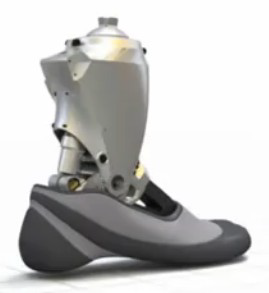
\includegraphics[width=.8\textwidth]{images/prot_01}
}%figues de la page de garde

\def\xxpied{%
DM 1 : Récursivité et Métrologie
}


\setcounter{secnumdepth}{5}
%---------------------------------------------------------------------------


\begin{document}
%\chapterimage{png/Fond_Cin}
\pagestyle{empty}


%%%%%%%% PAGE DE GARDE COURS
\ifcours
\begin{tikzpicture}[remember picture,overlay]
\node at (current page.north west)
{\begin{tikzpicture}[remember picture,overlay]
\node[anchor=north west,inner sep=0pt] at (0,0) {\includegraphics[width=\paperwidth]{\thechapterimage}};
\draw[anchor=west] (-2cm,-8cm) node [line width=2pt,rounded corners=15pt,draw=ocre,fill=white,fill opacity=0.6,inner sep=40pt]{\strut\makebox[22cm]{}};
\draw[anchor=west] (1cm,-8cm) node {\huge\sffamily\bfseries\color{black} %
\begin{minipage}{1cm}
\rotatebox{90}{\LARGE\sffamily\textsc{\color{ocre}\textbf{\xxnumpartie}}}
\end{minipage} \hfill
\begin{minipage}[c]{14cm}
\begin{titrepartie}
\begin{flushright}
\renewcommand{\baselinestretch}{1.1} 
\Large\sffamily\textsc{\textbf{\xxpartie}}
\renewcommand{\baselinestretch}{1} 
\end{flushright}
\end{titrepartie}
\end{minipage} \hfill
\begin{minipage}[c]{3.5cm}
{\large\sffamily\textsc{\textbf{\color{ocre} \discipline}}}
\end{minipage} 
 };
\end{tikzpicture}};
\end{tikzpicture}


\begin{tikzpicture}[overlay]
\node[shape=rectangle, 
      rounded corners = .25 cm,
	  draw= ocre,
	  line width=2pt, 
	  fill = ocre!10,
	  minimum width  = 2.cm,
	  minimum height = 2.5cm,] at (18cm,-4.7cm) {};
\node at (17.7cm,-4.65) {\rotatebox{90}{\textbf{\Large\color{ocre}{\classe}}}};
%{};
\end{tikzpicture}

\vspace{3.5cm}

\begin{tikzpicture}[remember picture,overlay]
\draw[anchor=west] (-2cm,-6cm) node {\huge\sffamily\bfseries\color{black} %
\begin{minipage}{2cm}
\begin{center}
\LARGE\sffamily\textsc{\color{ocre}\textbf{\xxactivite}}
\end{center}
\end{minipage} \hfill
\begin{minipage}[c]{15cm}
\begin{titrechapitre}
\renewcommand{\baselinestretch}{1.1} 
\Large\sffamily\textsc{\textbf{\xxnumchapitre}}

\Large\sffamily\textsc{\textbf{\xxchapitre}}
\vspace{.5cm}

\renewcommand{\baselinestretch}{1} 
\normalsize\normalfont
\xxcompetences
\end{titrechapitre}
\end{minipage}  };
\end{tikzpicture}
\vfill

\begin{flushright}
\begin{minipage}[c]{.3\linewidth}
\begin{center}
\xxfigures
\end{center}
\end{minipage}\hfill
\begin{minipage}[c]{.6\linewidth}
\startcontents
\printcontents{}{1}{}
\end{minipage}
\end{flushright}

\begin{tikzpicture}[remember picture,overlay]
\draw[anchor=west] (4.5cm,-.7cm) node {
\begin{minipage}[c]{.2\linewidth}
\begin{flushright}

\includegraphics[width=2cm]{png/logoCC}
\end{flushright}
\end{minipage}
\begin{minipage}[c]{.2\linewidth}
\textsl{\xxauteur} \\
\textsl{\classe}
\end{minipage}
 };
\end{tikzpicture}
\newpage
\pagestyle{fancy}

\newpage
\pagestyle{fancy}

\else
\fi


%%%%%%%% PAGE DE GARDE TD
\iftd
%\begin{tikzpicture}[remember picture,overlay]
%\node at (current page.north west)
%{\begin{tikzpicture}[remember picture,overlay]
%\draw[anchor=west] (-2cm,-3.25cm) node [line width=2pt,rounded corners=15pt,draw=ocre,fill=white,fill opacity=0.6,inner sep=40pt]{\strut\makebox[22cm]{}};
%\draw[anchor=west] (1cm,-3.25cm) node {\huge\sffamily\bfseries\color{black} %
%\begin{minipage}{1cm}
%\rotatebox{90}{\LARGE\sffamily\textsc{\color{ocre}\textbf{\xxnumpartie}}}
%\end{minipage} \hfill
%\begin{minipage}[c]{13.5cm}
%\begin{titrepartie}
%\begin{flushright}
%\renewcommand{\baselinestretch}{1.1} 
%\Large\sffamily\textsc{\textbf{\xxpartie}}
%\renewcommand{\baselinestretch}{1} 
%\end{flushright}
%\end{titrepartie}
%\end{minipage} \hfill
%\begin{minipage}[c]{3.5cm}
%{\large\sffamily\textsc{\textbf{\color{ocre} \discipline}}}
%\end{minipage} 
% };
%\end{tikzpicture}};
%\end{tikzpicture}

%%%%%%%%%% PAGE DE GARDE TD %%%%%%%%%%%%%%%
%\begin{tikzpicture}[overlay]
%\node[shape=rectangle, 
%      rounded corners = .25 cm,
%	  draw= ocre,
%	  line width=2pt, 
%	  fill = ocre!10,
%	  minimum width  = 2.5cm,
%	  minimum height = 2.5cm,] at (18.5cm,0) {};
%\node at (17.7cm,0) {\rotatebox{90}{\textbf{\Large\color{ocre}{\classe}}}};
%%{};
%\end{tikzpicture}

% PARTIE ET CHAPITRE
%\begin{tikzpicture}[remember picture,overlay]
%\draw[anchor=west] (-1cm,-2.1cm) node {\large\sffamily\bfseries\color{black} %
%\begin{minipage}[c]{15cm}
%\begin{flushleft}
%\xxnumchapitre \\
%\xxchapitre
%\end{flushleft}
%\end{minipage}  };
%\end{tikzpicture}

% Bandeau titre exo
\vspace*{\espacebandeautitre}
\begin{tikzpicture}[remember picture,overlay]
\draw[anchor=west] (-2cm,-6cm) node {\huge\sffamily\bfseries\color{black} %
\begin{minipage}{5cm}
\begin{center}
\LARGE\sffamily\color{ocre}\textbf{\textsc{\xxactivite}}

\begin{center}
\xxfigures
\end{center}

\end{center}
\end{minipage} \hfill
\begin{minipage}[c]{12cm}
\begin{titrechapitre}
\renewcommand{\baselinestretch}{1.1} 
\large\sffamily\textbf{\textsc{\xxtitreexo}}

\small\sffamily{\textbf{\textit{\color{black!70}\xxsourceexo}}}
\vspace{.5cm}

\renewcommand{\baselinestretch}{1} 
\normalsize\normalfont
\xxcompetences
\end{titrechapitre}
\end{minipage}  };
\end{tikzpicture}

\else
\fi


%%%%%%%% PAGE DE GARDE FICHE
\iffiche
\begin{tikzpicture}[remember picture,overlay]
\node at (current page.north west)
{\begin{tikzpicture}[remember picture,overlay]
\draw[anchor=west] (-2cm,-3.25cm) node [line width=2pt,rounded corners=15pt,draw=ocre,fill=white,fill opacity=0.6,inner sep=40pt]{\strut\makebox[22cm]{}};
\draw[anchor=west] (1cm,-3.25cm) node {\huge\sffamily\bfseries\color{black} %
\begin{minipage}{1cm}
\rotatebox{90}{\LARGE\sffamily\textsc{\color{ocre}\textbf{\xxnumpartie}}}
\end{minipage} \hfill
\begin{minipage}[c]{14cm}
\begin{titrepartie}
\begin{flushright}
\renewcommand{\baselinestretch}{1.1} 
\large\sffamily\textsc{\textbf{\xxpartie} \\} 

\vspace{.2cm}

\normalsize\sffamily\textsc{\textbf{\xxnumchapitre -- \xxchapitre}}
\renewcommand{\baselinestretch}{1} 
\end{flushright}
\end{titrepartie}
\end{minipage} \hfill
\begin{minipage}[c]{3.5cm}
{\large\sffamily\textsc{\textbf{\color{ocre} \discipline}}}
\end{minipage} 
 };
\end{tikzpicture}};
\end{tikzpicture}


\begin{tikzpicture}[overlay]
\node[shape=rectangle, 
      rounded corners = .25 cm,
	  draw= ocre,
	  line width=2pt, 
	  fill = ocre!10,
	  minimum width  = 2.5cm,
	  minimum height = 2.5cm,] at (18.5cm,-.6cm) {};
\node at (17.8cm,-.6cm) {\rotatebox{90}{\textsf{\textbf{\large\color{ocre}{\classe}}}}};
%{};
\end{tikzpicture}



\else
\fi



\vspace{2cm}
\pagestyle{fancy}
\thispagestyle{plain}

\section{Exercice}

On considère la fonction suivante :\\
\begin{python}
def f(x) :
    if x <= 1 :
	return 1
    elif x % 2 == 0 :
	return 2*f(x/2)
    else :
	return 1 + f(x+1)
\end{python}

\begin{enumerate}
\item Montrer que cette fonction récursive se termine pour toute valeur entière 
de l'argument \texttt{x}.
\item Soient $x\in\mathbb N$ et $g(x)=f(x)+x$. À partir du programme précédent, donner 
un programme python qui calcule $g(x)$.
\item En déduire que pour tout $x\in\mathbb N$, $g(x)$ est une puissance de 2.
\end{enumerate}

\ifprof
\section*{Corrigé }

\begin{enumerate}
\item Si $x$ est pair et $> 1$, alors $f (x) = 2f (x/2)$ et $ x/2 < x$. Si $x$ est impair et
 $ > 1$, alors $f (x) = 1 + 2f ((x + 1)/2)$ et $(x + 1)/2 < x$. Donc dans les deux cas
     récursifs, on appelle $f$ en une ou deux étapes avec un argument strictement
     inférieur à $x$. Ceci prouve la terminaison du calcul de $f (x)$ par récurrence
     sur $x$.
\item Soit $g(x) = f (x) + x$. En remplaçant $f (x)$ par $g(x)- x$ dans la définition de
    $ $f et en simplifiant, on obtient un programme calculant $g$ :\\
    
   
\begin{python}
def g(x) :
    if x <= 1 :
	return 1 + x
    elif x % 2 == 0 :
	return 2*g(x/2)
    else :
	return g(x+1)
\end{python} 

\item Avec la question précédente, il est immédiat par récurrence que $g(x)$ est toujours une puissance de 2.

 \end{enumerate}

\else
\fi

\section{Métrologie}
\subsection{Mise en situation}
\ifprof
\else

\noindent\begin{minipage}[c]{.75\linewidth}
La métrologie est la << science des mesures >>. Dans l'industrie, elle désigne les opération permettant de valider ou non les dimensions et les formes des pièces fabriquées. On peut par exemple vérifier qu'une mesure dimensionnelle vérifie le cahier des charges. On peut aussi vérifier qu'une surface plane fabriquée vérifie le cahier des charges (on parle alors de planéité).

Pour vérifier les pièces, on utilise une machine à mesurer tridimensionnelle (image ci-contre) qui permet de palper des points et de les stocker afin de les analyser.

\end{minipage} \hfill
\begin{minipage}[c]{.2\linewidth}
\begin{center}
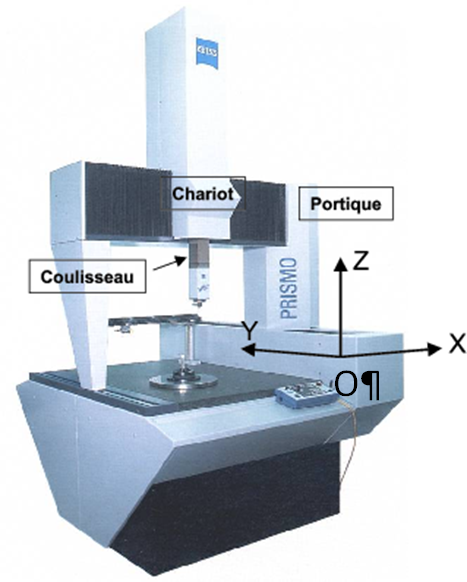
\includegraphics[width=.95\textwidth]{images/MMT}
\end{center}
\end{minipage}

En métrologie, il peut être est nécessaire de construire un plan idéal à partir d'un nuage de points palpés. Un des critères de construction prévu par la norme et de construire un <<plan tangent extérieur à la matière qui minimise l'écart maximum >>. Dans la pratique, il est assez difficile de calculer le plan optimal. 


\begin{center}
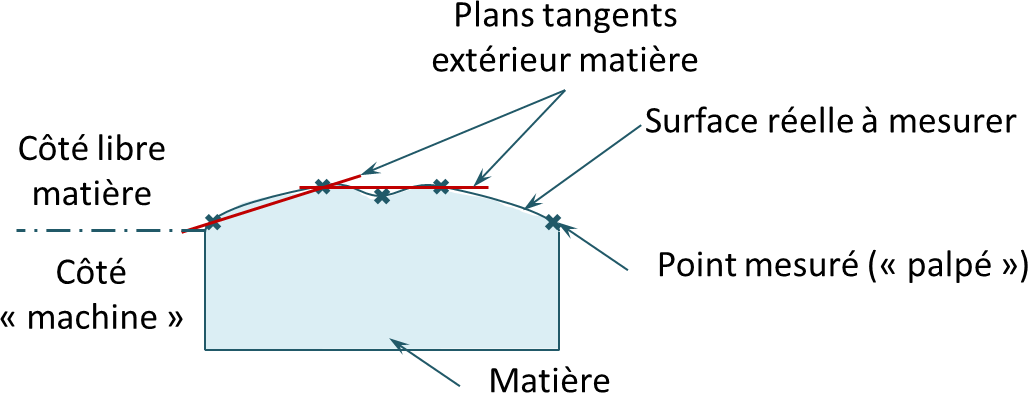
\includegraphics[width=.7\textwidth]{images/plan_tgt}
\end{center}

\begin{obj}
L'objectif de ce travail est de déterminer algorithmiquement, de manière approchée, le plan tangent extérieur matière qui minimise l'écart maximum. 
\end{obj}
\fi




\subsection{Mise en équation de détermination du plan des moindre carrés}
\ifprof
\else

On suppose que la direction de mesure $\vect{z}$ est verticale ascendante pour la machine à mesurer tridimensionnelle. En conséquence, on traitera les plans qui ne contiennent pas le vecteur $\vect{z}$.

\begin{rappel} ~\\ \vspace{-.25cm}

Dans un repère orthonormé direct, l'équation d'un plan $\left( \mathcal{P}\right)$ est donnée par $z=ax+by+c$.

Le vecteur $\vect{n}(a,b,1)$ définit une normale au plan $\left( \mathcal{P}\right)$.

Le point de coordonnées $(0,0,c)$ appartient au plan $\left( \mathcal{P}\right)$.

\end{rappel}



L'écart $e_i$ d'un point  $M_i$ suivant $\vect{z}$ de coordonnées $\left(x_i,y_i,z_i\right)$ au plan $\left( \mathcal{P}\right)$ est donné par 
$e_i = z_i -ax_i -by_i -c$.
On remarquera que $e_i$ est, à une constante multiplicative près, la distance algébrique du point $M_i$ au plan $\mathcal{P}$.

\begin{defi}\textbf{Écarts}
La fonction écart $E$ est définie de la manière suivante : 
$$
E:(a,b,c)\rightarrow \sum\limits_{i=1}^{n} e_i^2 = \sum\limits_{i=1}^{n} \left(z_i -ax_i -by_i -c\right)^2
$$
\end{defi}


\begin{defi}\textbf{Minimisation des écarts}

Pour minimiser la fonction $E$, il faut résoudre le système d'équations suivant :

\begin{tabular}{p{4cm}p{4cm}p{4cm}}
\begin{eqnarray}\label{eq1}
\dfrac{\partial E(a,b,c)}{\partial a} = 0 
\end{eqnarray}
&
\begin{eqnarray}\label{eq2}
\dfrac{\partial E(a,b,c)}{\partial b} = 0 
\end{eqnarray}
&
\begin{eqnarray}\label{eq3}
\dfrac{\partial E(a,b,c)}{\partial c} = 0 
\end{eqnarray}% \\
\end{tabular}

\end{defi}



\begin{rappel} ~\\ \vspace{-.25cm}

On remarque que la méthode des moindres carrés ne minimise pas la somme des écarts $e_i$ mais celle de leur carré. On pourrait vérifier que minimiser la fonction $E':(a,b,c)\rightarrow \sum\limits_{i=1}^{n} e_i$ à l’aide des relations obtenues par dérivations partielles, ne permettrait pas de déterminer les valeurs de $a$, $b$ et $c$.
\end{rappel}


\fi
\section{Détermination du défaut de planéité}

\begin{obj}
L'objectif de cette partie est de rechercher le plan des moindres carrés c'est à dire de trouver les valeurs $a$, $b$ et $c$ qui minimisent les écarts entre le plan $\mathcal{P}$ et un nuage de points. 

Le plan des moindre carrés permettra de déterminer le défaut de planéité.
\end{obj}

\subsection{Conditionnement du problème}

\subparagraph{}
\textit{Montrer que la méthode des moindres carrés permet d'aboutir aux 3 équations suivantes :}

$$
\sum\limits_{i=1}^n \left(ax_i^2 + bx_i y_i  +c x_i -x_i z_i  \right) = 0 \quad 
\sum\limits_{i=1}^n  \left(ax_iy_i  + by_i^2 +cy_i -y_i z_i  \right) = 0 \quad 
\sum\limits_{i=1}^n  \left(ax_i +  by_i+c -z_i  \right) = 0
$$

\ifprof
\begin{corrige}

On a : 

$\dfrac{\partial E(a,b,c)}{\partial a} = 0 
\Leftrightarrow  \sum\limits_{i=1}^{n} \dfrac{\partial \left(z_i -ax_i -by_i -c\right)^2}{\partial a}  = 0
\Leftrightarrow   \sum\limits_{i=1}^{n} -2x_i  \left(z_i -ax_i -by_i -c\right)  = 0
$

Au final:  $\dfrac{\partial E(a,b,c)}{\partial a} = 0 
\Leftrightarrow   \sum\limits_{i=1}^{n}   \left(-x_iz_i +ax_i^2 +bx_i y_i +cx_i\right) = 0$

On a :

$\dfrac{\partial E(a,b,c)}{\partial b} = 0
\Leftrightarrow \sum\limits_{i=1}^{n} \dfrac{\partial \left(z_i -ax_i -by_i -c\right)^2}{\partial b}  =0 
\Leftrightarrow \sum\limits_{i=1}^{n} -2y_i  \left(z_i -ax_i -by_i -c\right) = 0
$

Au final : $\dfrac{\partial E(a,b,c)}{\partial b} = 0 
\Leftrightarrow   \sum\limits_{i=1}^{n}     \left(-y_iz_i + ax_i y_i  +by_i^2 +cy_i\right)  = 0$


On a :

$\dfrac{\partial E(a,b,c)}{\partial c} = 0
\Leftrightarrow \sum\limits_{i=1}^{n} \dfrac{\partial \left(z_i -ax_i -by_i -c\right)^2}{\partial c}  =0 
\Leftrightarrow \sum\limits_{i=1}^{n} -2  \left(z_i -ax_i -by_i -c\right) = 0
$

Au final : $\dfrac{\partial E(a,b,c)}{\partial b} = 0 
\Leftrightarrow   \sum\limits_{i=1}^{n}  \left(-z_i +ax_i +by_i +c\right) = 0$

\end{corrige}

\else
\fi

\vspace{.5cm}
On définit les grandeurs suivantes : 

$S_{xx} = \sum\limits_{i=1}^n x_i^2$, $S_{yy} = \sum\limits_{i=1}^n y_i^2$, $S_{xy} = \sum\limits_{i=1}^n x_i y_i$, $S_{xz} = \sum\limits_{i=1}^n x_i z_i$, $S_{yz} = \sum\limits_{i=1}^n y_i z_i$, 
$S_x  = \sum\limits_{i=1}^n  x_i$, $S_y  = \sum\limits_{i=1}^n  y_i$ et $S_z  = \sum\limits_{i=1}^n  z_i $.

%\begin{center}
%\begin{tabular}{ccc}
%$S_{xx} = \sum\limits_{i=1}^n x_i^2$ && $S_{yy} = \sum\limits_{i=1}^n y_i^2$  \\
%$S_{xy} = \sum\limits_{i=1}^n x_i y_i$ & $S_{xz} = \sum\limits_{i=1}^n x_i z_i$ & $S_{yz} = \sum\limits_{i=1}^n y_i z_i$  \\
%$S_x  = \sum\limits_{i=1}^n  x_i$ & $S_y  = \sum\limits_{i=1}^n  y_i$ & $S_y  = \sum\limits_{i=1}^n  x_i $\\
%\end{tabular}
%\end{center}

On note $X=(a,b,c)$ le vecteur solution du problème avec $X\in \mathcal{M}_{1,3} \left(\mathbb{R} \right)$.


\subparagraph{}
\textit{Montrer que le problème peut se mettre sous la forme du système linéaire suivant : $AX + B = 0$  où $A \in \mathcal{M}_{3,3} \left(\mathbb{R} \right)$ et  $B \in \mathcal{M}_{1,3} \left(\mathbb{R} \right)$. On donnera les expressions de $A$ et de $B$.}

\ifprof
\begin{corrige}
On a : 
$$
\sum\limits_{i=1}^{n}   \left(-x_iz_i +ax_i^2 +bx_i y_i +cx_i\right) = 0 
\Leftrightarrow    - \sum\limits_{i=1}^{n} x_iz_i +\sum\limits_{i=1}^{n}ax_i^2 +\sum\limits_{i=1}^{n}bx_i y_i +\sum\limits_{i=1}^{n}cx_i  = 0 
$$
$$
\Leftrightarrow    a\sum\limits_{i=1}^{n}x_i^2 +b\sum\limits_{i=1}^{n}x_i y_i +c\sum\limits_{i=1}^{n}x_i  = \sum\limits_{i=1}^{n} x_iz_i
\Leftrightarrow    aS_{xx} +bS_{xy} +cS_x  =S_{xz}
$$
De même, on détermine que : 
$$
\sum\limits_{i=1}^{n}     \left(-y_iz_i + ax_i y_i  +by_i^2 +cy_i\right)  = 0
\Leftrightarrow aS_{xy} + bS_{yy}+cS_y = S_{yz}
$$

$$
\sum\limits_{i=1}^{n}  \left(-z_i +ax_i +by_i +c\right) = 0
\Leftrightarrow aS_{x} + bS_{y}+cn = S_{z}
$$
On a donc : 
$$
\left\{
\begin{array}{l}
aS_{xx} +bS_{xy} +cS_x  =S_{xz} \\
aS_{xy} + bS_{yy}+cS_y = S_{yz} \\
aS_{x} + bS_{y}+cn = S_{z}
\end{array}
\right.
\Leftrightarrow
\left[ 
\begin{array}{ccc}
S_{xx} & S_{xy} & S_x \\
S_{xy} & S_{yy} & S_y \\
S_{x} & S_{y} & n \\
\end{array}
\right]
\cdot 
\left[ 
\begin{array}{c}
a \\b \\ c\end{array}
\right]
=
\left[ 
\begin{array}{c}
S_{xz} \\
S_{yz} \\ 
S_{z}\end{array}
\right]
\Leftrightarrow
AX = -B
$$

Le signe négatif provient de la formulation du problème dans la question. 

\end{corrige}

\else
\fi


\subsection{Résolution du problème}
\ifprof
\else
\begin{methode}
Au final, pour déterminer le plan des moindres carrés, la démarche est la suivante :
\begin{itemize}
\item mesurer les points$(x_i,y_i,z_i)$ grâce à la machine à mesurer et exporter les données dans un fichier (ici un fichier texte);
\item importer le fichier de points avec Python;
\item résoudre le système linéaire $AX+B=0$ pour déterminer $a$, $b$ et $c$ permettant d'obtenir l'équation du plan. 
\end{itemize}
\end{methode}
\fi

\subparagraph{}
\textit{Donner une méthode (ou le nom d'un algorithme) permettant de résoudre le système linéaire ci-dessus. Préciser les différentes étapes de cet algorithme ainsi que sa complexité.}


\ifprof
\begin{corrige}
Pour résoudre ce problème, il est possible d'utiliser l'algorithme du pivot de Gauss. Cet algorithme se déroule en trois phases majeures : 
\begin{enumerate}
\item recherche du pivot;
\item triangularisation de la matrice $A$ (en phase avec les transformations nécessaires sur la matrice $B$);
\item phase de remontée permettant de déterminer $X$. 
\end{enumerate}

On peut montrer que la complexité algorithmique du pivot de Gauss est en $\mathcal{O}\left(n^3\right)$.
\end{corrige}
\else
\fi
\ifprof
\else
\vspace{.5cm}

Les points mesurés par une machine à mesurer tridimensionnelle sont stockés dans un fichier texte. Dans ce fichier sont inscrits successivement les coordonnés des points puis les coordonnées de la normale de contact entre le palpeur et la surface mesurée. Le fichier est de la forme suivante : 

\begin{tabular}{l}
\texttt{-101.88340,-155.21568,-50.30434,0,0,1}\\
\texttt{-99.21040,-145.54768,-50.304844,0,0,1}\\
\texttt{-82.43090,-129.69318,-50.292844,0,0,1}\\
\texttt{-59.72540,-134.12818,-50.301844,0,0,1}\\
\texttt{...} \\
\end{tabular}

\begin{rem}
La fonction \texttt{split} permet de séparer les éléments d'une chaîne de caractère suivant un motif et de les stocker dans une liste :
\begin{python}
>>> a = "-101.88340,-155.21568,-50.30434,0,0,1"
>>> a = a.split(",")
           ['-59.72540', '-134.12818', '-50.301844', '0', '0', '1']
\end{python}
\end{rem}
\fi

\subparagraph{}
\textit{Donner l'implémentation de la fonction \texttt{read\_file} permettant de lire un fichier de mesures formaté comme indiqué ci-dessus et permettant de retourner la liste des points mesurés.}
\vspace{.5cm}

\ifprof
\begin{corrige}
~\\
\begin{python}
def read_file(file):
    fid = open(file,'r')
    pts=[]
    for ligne in fid:
        ligne = ligne.split(",")
        print(ligne)
        pts.append([float(ligne[0]),float(ligne[1]),float(ligne[2])])
    return pts
\end{python}
\end{corrige}
\else
\fi

\ifprof
\else

On appelle \texttt{plan\_moindres\_carres} la fonction permettant de trouver la solution du système linéaire à partir d'une liste de points. Ces spécifications sont les suivantes :
\begin{py}
\begin{python}
def plan_moindres_carres(liste_pts):
    """
    Permet de déterminer les caractéristiques du plan des moindres carrés.
    Entrée : 
        * liste_pts (list) : liste de points de la forme [[x1,y1,z1],[x2,y2,z2],...]
    Sortie : 
        * pl(list) : solution du problème d'optimisation : retourne [a,b,c]
    """
\end{python}
\end{py}
\fi

\subparagraph{}
\textit{Donner l'implémentation du programme principal (main) permettant de lire le fichier de mesure appelé \texttt{mesures.txt} et de déterminer la liste des paramètres \texttt{[a,b,c]} correspondant aux paramètres du plan des moindres carrés. Vous utiliserez les fonctions précédemment définies.}
\ifprof
\begin{corrige}~\\
\begin{python}
liste_pts=read_file("mesures.txt")
plan = plan_moindres_carres(liste_pts)
\end{python}
\end{corrige}
\else
\fi


\subsection{Application -- Détermination du défaut de planéité}

\ifprof
\else

Pour déterminer le défaut de planéité d'une forme, il est nécessaire de déterminer la distance maximale entre les points les plus éloignés de part et d'autre du plan des moindres carrés.

\begin{center}
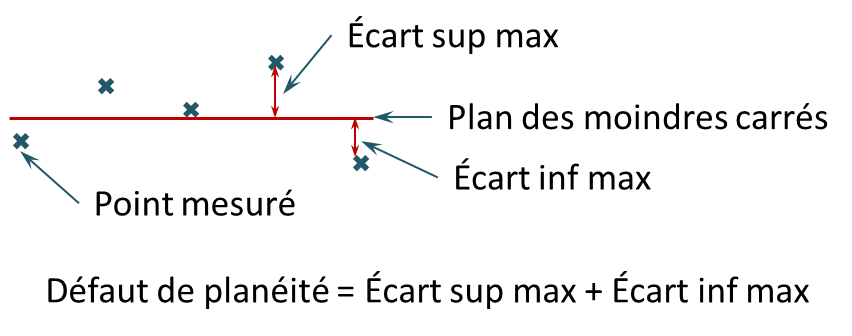
\includegraphics[width=.7\linewidth]{images/planeite_2}
\end{center}
On définit la distance algébrique $d$ d'un point $M$ de coordonnées $\left(x,y,z\right)$ au plan $\left( \mathcal{P}\right)$ par l'expression suivante :
$d = \dfrac{z - a x -b y -c}{\sqrt{a^2+b^2+1}}$.

On notera \texttt{pt} la liste contenant les coordonnées d'un point et \texttt{pl} la liste contenant le triplet \texttt{(a,b,c)}.

\fi 

\subparagraph{}
\textit{Donner l'implémentation de la fonction  \texttt{dist\_pt\_plan} en Python permettant de retourner la distance algébrique entre un point et un plan. Les spécifications de la fonction sont les suivantes :}
\begin{py}
\begin{python}
def dist_pt_plan(pt,plan):
    """
    Permet de calculer une distance point - plan
    Entrées : 
        * pt(list) : point de coordonnées [x,y,z]
        * plan(list) : caractéristiques du plan [a,b,c]
    Sortie : 
        * d(flt) : distance
    """
\end{python}
\end{py}
\ifprof
\begin{corrige}~\\
\begin{python}
def dist_pt_plan(pt,pl):
    return (pt[2]-pl[0]*pt[0]-pl[1]*pt[1]-pl[2])/(sqrt(pl[0]**2+pl[1]**2+1))
\end{python}
\end{corrige}
\else
\fi

\subparagraph{}
\textit{Donner l'implémentation de la fonction \texttt{defaut\_planeite} en Python permettant de retourner le défaut de planéité. On donne les spécifications de la fonction : }
\begin{py}
\begin{python} 
def defaut_planeite(pl,liste_pt):
    """
    Permet de calculer une distance point - plan
    Entrées : 
        * pl(list) : caractéristiques du plan [a,b,c]
        * liste_pts (list) : liste de points de la forme [[x1,y1,z1],[x2,y2,z2],...]
        
    Sortie : 
        * d(flt) : distance
    """
\end{python}
\end{py}
\ifprof
\begin{corrige}~\\
\begin{python}
def defaut_planeite(pl,liste_pt):
    dist_p=0
    dist_n=0
    for i in range(len(liste_pt)):
        dist=dist_pt_plan(liste_pt[i],pl)
        if dist_p<dist and dist>0 :
            dist_p=dist
        elif dist_n>dist and dist<0 :
            dist_n=dist
    return dist_p-dist_n
\end{python}
\end{corrige}
\else
\fi

\section{Construction d'une référence spécifiée associée à une surface nominalement plane}

\ifprof
\else

Pour associer un plan idéal à un nuage de points, la norme prévoit de lui associé un plan tangent extérieur matière minimisant les écarts. Mathématiquement, ce problème n'est pas simple à résoudre. Afin d'approcher la solution, on se propose d'utiliser, dans le cadre ce travail,  la méthode suivante : 

\begin{methode}
~\\
\begin{enumerate}
\item Détermination du plan par la méthode des moindres carrés.
\item Translation du plan au point le plus éloigné côté libre de la matière.
\item Balancement du plan afin de minimiser les défauts : on fait varier son orientation.
\item Vérification que tous les points sont situés sous le plan.
\item Changement au point le plus éloigné situé côté libre de la matière s'il y en a.
\end{enumerate}
Les étapes 4 et 5 peuvent être itératives.
\begin{warn}
\textbf{\textsf{Attention :}} les points 3, 4 et 5 ne sont qu'une piste envisagée dans le cadre de ce travail et ne constituent pas un algorithme utilisé dans les logiciels de mesure.
\end{warn}
\end{methode}

\newpage 

On donne la fonction suivante :

\begin{py}
\begin{python}
def mystere(pl,liste_pt):
    ind=0
    d=dist_pt_plan(liste_pt[ind],pl)
    for i in range(1,len(liste_pt)):
        temp=dist_pt_plan(liste_pt[i],pl)
        if temp>d :
            ind=i
            d=dist_pt_plan(liste_pt[ind],pl)
    return ind
\end{python}
\end{py}

\fi 

\subparagraph{}
\textit{Quel est l'objectif de cette fonction ? En déduire le triplet correspondant à l'équation du plan répondant au point \textbf{2} de la méthode. }
\ifprof
\begin{corrige}
Cette fonction a pour but de retrouver l'indice du point étant le plus éloigné du plan des moindres carrés. Ce point est aussi du coté libre de la matière.

Le nouveau plan a donc pour caractéristiques : 

\texttt{[a,b,liste\_pt[ind][2]-X[0]*liste\_pt[ind][0]-X[1]*liste\_pt[ind][1]}.
\end{corrige}
\else
\fi

\ifprof
\else
Le balançage du plan par rapport à un point est réalisé grâce à la fonction suivante. 

\begin{py}
\begin{python}
def balancage(pl, pt):
    npt=25
    pas=0.000003
    dist=100000
    pl2=[None,None,None]
    for k in range(-npt,npt):
        pl2[0]=pl[0]+k*pas
        for j in range(-npt,npt):
            pl2[1]=pl[1]+j*pas
            pl2[2]=pt[2]-pl2[0]*pt[0]-pl2[1]*pt[1]
            temp=defaut_planeite(pl2,liste_pt)	
            if temp<dist :
                dist=temp
                f=pl2[0]
                g=pl2[1]
                h=pl2[2]
    pl2=[f,g,h]    
    return [pl2,dist]	
\end{python}
\end{py}

\fi

\subparagraph{}
\textit{Quel est l'objectif de cette fonction ? Que retourne-t-elle ? Donner un commentaire pour chacune des instructions.}
\ifprof
\begin{corrige}
~\\
\begin{minipage}[c]{.57\linewidth}
\begin{python}
 1. def balancage(pl, pt):
 2.    npt=25                            #
 3.    pas=0.000003                      #
 4.    dist=100000                       #
 5.    pl2=[None,None,None]              #
 6.    for k in range(-npt,npt):         #
 7.        pl2[0]=pl[0]+k*pas            #
 8.        for j in range(-npt,npt):     #
 9.            pl2[1]=pl[1]+j*pas        #
10.            pl2[2]=pt[2]-pl2[0]*pt[0]-pl2[1]*pt[1]  #
11.            temp=defaut_planeite(pl2,liste_pt)	   #
12.            if temp<dist :         #
13.                dist=temp          #
14.                f=pl2[0]           #
15.                g=pl2[1]           #
16.                h=pl2[2]           #
17.    pl2=[f,g,h]                    #    
18.    return [pl2,dist]	      #
\end{python}
\end{minipage}\hfill
\begin{minipage}[c]{.43\linewidth}
L'objectif de cette fonction est de déterminer une référence spécifiée en faisant varier l'orientation du plan des moindres carrés. Elle retourne le plan optimal ainsi que le défaut de planéité lié au nuage de point.

Les boucles \textsl{for} lignes 6 et 8 permettent de réaliser des petite variation autour d'un point \textsl{pt} prédéterminé. 
Ligne 10 on dispose alors des caractéristiques d'un plan ayant subi deux petites rotations. 
On détermine alors le défaut de planéité lié à ce nouveau plan. 

On cherche alors le nouveau plan << minimisant le défaut de planéité >> (en fait on ne minimise pas le défaut mais l'écart...).

\end{minipage}
\end{corrige}
\else
\fi

\subparagraph{}
\textit{Quelle est la complexité de cet algorithme si on cherche à améliorer le choix du plan optimal par rapport à un seul des points du nuage de points ? Comment évolue la complexité de ce programme si on cherche à réaliser le balançage en utilisant chacun des points mesurés ?}
\ifprof
\begin{corrige}
Pour avoir une <<meilleure>> solution du problème, on peut augmenter le nombre de pas de calcul. Les deux boucles imbriquées dépendant du nombre de points, on a une complexité en $\mathcal{O}(npt^2)$.

On note $n$ le nombre points palpés. Si on réalise un balançage sur chacun des points du nuage, la complexité sera en $\mathcal{O}(n\cdot npt^2)$
\end{corrige}
\else
\fi


\end{document}